Many algorithms and tools in robotic autonomy leverage models of the world that are often based on first-principles: physics-based kinematic models are used to design controllers, sensor models are used in localization algorithms, and geometric principles are used in understanding stereo vision. However, there are also many scenarios in robotics where these techniques may fail to capture the complexity of unstructured real-world environments. For example, how can a stop-sign be reliably detected in camera images when it could be rainy, foggy, or dark out, or when the stop-sign is partially occluded? Are there first-principles models that can accurately predict the behavior of a human driver, and distinguish between aggressive and defensive driving behavior? How can a robot be programmed to pick up objects with an infinite number of variations in size, shape, color, and texture? In the last few decades, advancements in \textit{machine learning}\cite{HastieTibshiraniEtAl2017} have led to start-of-the-art approaches for many of these challenging problems\footnote{Of course in many settings it is beneficial to use first-principles and machine learning techniques \textit{in concert}.}. This chapter presents an introduction to machine learning to provide a knowledge of the fundamental tools that are used in learning-based algorithms for robotics, including computer vision, reinforcement learning, and more.

\notessection{Machine Learning}
At their most fundamental level, machine learning techniques seek to extract useful patterns from \textit{data}\footnote{In many cases the data will come from real world experiments, but in other cases may come from simulation.}, and are typically classified as either \textit{supervised} or \textit{unsupervised}.

\begin{definition}[Supervised Learning]
Given a collection of $n$ data points:
\begin{equation*}
\{(x_1, y_1), \dots, (x_n, y_n)\},    
\end{equation*}
where $x_i$ is an input variable and $y_i$ is an output, the \textit{supervised learning} problem is to find a function $y = f(x)$ that fits the data and can be used to predict outputs $y$ for new inputs $x$. 
\end{definition}

\begin{definition}[Unsupervised Learning]
Given a collection of $n$ data points $\{x_1, \dots, x_n\}$, the \textit{unsupervised learning} problem is to find patterns in the data.
\end{definition}

Supervised learning problems, such as regression and classification\footnote{In regression problems the output $y$ is continuous and in classification problems the output $y$ is discrete (categorical).}, are generally more common in robotics applications and will be the focus of this chapter. For example, robotic imitation learning-based controllers\footnote{Imitation learning refers to the process of learning to mimic a policy (e.g. from an expert) through example decisions.} can be expressed as a regression problem where the input $x$ is the state of the robot and $y$ is the action the robot should take. Classification problems also arise frequently in robotic computer vision, for example to identify whether the image $x$ belongs to a particular class $y$ (e.g. a dog or cat).

In both regression and classification problems, the learned function $f$ is categorized as either \textit{parametric} or \textit{non-parametric}. Parametric functions are generally more structured and can be written down in an analytical form\footnote{The most basic parametric function would be a linear function $f(x) = Wx$, parameterized by the ``weight'' matrix $W$.}, while non-parametric functions are generally defined by the data points themselves\footnote{In the non-parametric k-nearest neighbors method, the value $f(x)$ is defined by the value of the data points $y_i$ corresponding to the $k$ closest points, $x_i$, to $x$.}. The best choice between parametric or non-parametric functions is generally dependent on the particular problem and the type of data available. However, some of the most popular choices are parametric, such as polynomials and \textit{neural networks}.

\subsection{Loss Functions}
In supervised learning problems, a metric known as a \textit{loss function} is used to evaluate and compare candidate models $f(x)$ that could be used to fit the data. Many loss functions for supervised learning problems exist, but some of the most common examples include the $l_2$ and $l_1$ loss (for regression) and the $0 - 1$ and cross entropy loss (for classification).

\begin{enumerate}
\item The $l_2$ loss function is defined by:
\begin{equation} \label{eq:l2loss}
L = \frac{1}{n}\sum_{i=1}^n ( f(x_i) - y_i )^2,
\end{equation}
where the summation is over some set of data points $(x^i, y^i)$. From this loss function it can be seen that a penalty arises from the function $f$ not perfectly matching the data at the sampled data points, but most importantly that the penalty is \textit{quadratic} with respect to this residual. This loss function will therefore favor more small residuals over a few large residuals, which tends to make the model perform better ``on average''. However this also makes the $l_2$ loss sensitive to outliers in the data, making the training less robust.
\item The $l_1$ loss function is defined by:
\begin{equation}
L = \frac{1}{n}\sum_{i=1}^n \lvert f(x_i) - y_i \rvert.
\end{equation}
Unlike the $l_2$ loss, this loss function only penalizes the \textit{absolute value} of the residual. Therefore this loss function will favor all residuals on a more equal footing and generally leads to a more robust training procedure that is less sensitive to outliers in the data.
\item The $0-1$ loss function is defined by:
\begin{equation}
L = \frac{1}{n}\sum_{i=1}^n \mathbf{1}\{f(x_i) \neq y_i \},
\end{equation}
where $\mathbf{1}\{\cdot\}$ is the indicator function.
This loss function can be used in classification problems and provides a loss of $1$ whenever the classification is incorrect, and $0$ otherwise. However, the use of this loss function introduces practical issues when training with gradient-based optimization, since this function is either flat or not differentiable at all points in the domain.
\item The cross entropy loss function\footnote{Cross entropy loss is more practical than $0-1$ loss since it is a differentiable function.} is defined by:
\begin{equation}
L = -\frac{1}{n}\sum_{i=1}^n y^\top_i \log f(x_i),
\end{equation}
and is a common loss function in classification problems. To get an intuitive feeling for how the cross entropy loss works, consider a classification problem where the classes are $c \in \{1, 2, \dots, C\}$ and where the function $f(x_i)$ outputs a \textit{vector} of the probabilities of each class (which is normalized to sum to $1$)\footnote{This can be accomplished by using the \textit{softmax} function.}. Additionally, for each data point the vector $y_i$ is a ``one-hot'' vector\footnote{A one-hot vector is a vector with all zeros and a single $1$.} specified by the class associated with $x_i$. Therefore the loss for a particular data point can be written as:
\begin{equation*}
-y^\top_i \log f(x_i) = -\begin{bmatrix}
0, \dots, 1, \dots, 0
\end{bmatrix}\begin{bmatrix}
\log f_1(x_i) \\ \vdots \\ \log f_C(x_i)
\end{bmatrix} = -\log f_c(x_i),
\end{equation*}
where $C$ is the number of classes, the $1$ element in $y_i$ is in the position corresponding to the correct class, and $f_c(x_i)$ is the probability of the correct class output by the model. Thus, to minimize the loss for this particular data point it is good to make $f_c(x_i) = 1$ (in fact as $f_c(x_i)\xrightarrow{} 0$ the loss approaches infinity!).
Cross entropy loss can also be derived from a statistical perspective, where it can be shown to be the same as maximizing the log-likelihood over all data points.
\end{enumerate}

\subsection{Model Training}
In supervised learning problems with a predetermined parametric model (e.g. linear model or neural network), the \textit{values} of the parameters can be optimized to best fit the data (i.e. minimize the specified loss function). This process of parameter optimization is referred to as \textit{model training}. While in some special cases the optimal set of parameters can be computed analytically, it is more common to search for a good set of parameters in an iterative fashion using numerical optimization techniques.

\begin{example}[Linear Least Squares]
One of the most fundamental regression problems, linear least squares, can be solved analytically. In this problem, the parametric model is a linear model\footnote{This approach can also be extended to nonlinear settings through the use of basis functions. In particular the model becomes $f(x) = \theta^\top \phi(x)$, where $\phi(x)$ are nonlinear basis functions (sometimes referred to as \textit{features}.}:
\begin{equation*}
    f(x) = \theta^\top x,
\end{equation*}
where $x \in \R^p$ is the input and $\theta \in R^p$ is the set of model parameters, and the loss function is the $l_2$ loss \eqref{eq:l2loss}. Given $n$ data points $(x_i, y_i)$, the loss function can be expressed in matrix form as:
\begin{equation*}
L(\theta) = \frac{1}{n}\lVert Y - X\theta \rVert_2^2,
\end{equation*}
where the matrix $Y \in \R^n$ and $X \in \R^{n \times p}$ are defined by the data as:
\begin{equation*}
Y = \begin{bmatrix}
y_1 \\ \vdots \\ y_n
\end{bmatrix}, \quad X = 
\begin{bmatrix}
x_1^\top \\ \vdots \\ x^\top_n
\end{bmatrix}.
\end{equation*}
The parameters $\theta$ are then chosen to minimize the loss function by taking the derivative:
\begin{equation*}
\frac{dL}{d\theta} = \frac{2}{n}X^\top X\theta - \frac{2}{n}X^\top Y,
\end{equation*}
and setting it equal to zero, which gives $\theta^* = (X^\top X)^{-1}X^\top Y$.\footnote{Note that directly computing the inverse of $X^\top X$ may be challenging, but alternative numerical methods exist to compute the value of $\theta^*$ that satisfies the necessary condition of optimality.}
\end{example}


\subsubsection{Numerical Optimization} \label{subsubsec:MLnumopt}
In many cases parameter optimization cannot be performed analytically and therefore numerical optimization algorithms are used. Two of the most fundamental algorithms for numerical optimization-based training of parametric models are \textit{gradient descent} and \textit{stochastic gradient descent}\footnote{Gradient descent is referred to as a \textit{first-order} method.}. 

In gradient descent, the parameters $\theta \in \R^p$  of a model $f_\theta(x)$ are iteratively updated by:
\begin{equation*}
\theta \xleftarrow{} \theta - \eta \nabla_\theta L(\theta),
\end{equation*}
where $\nabla_\theta L(\theta)$ is the gradient of the loss function with respect to the parameters and the hyperparameter $\eta$ is referred to as the \textit{learning rate} or \textit{step-size}. By leveraging the gradient, this update rule seeks to iteratively improve the parameters to incrementally decrease the loss.

Notice that the gradient of the loss can be written as:
\begin{equation*}
\nabla_\theta L(\theta) = \frac{1}{n}\sum_{i=1}^n \nabla_\theta L_i(\theta),   
\end{equation*}
where $L_i$ is the term of the loss function associated with the $i$-th data point.
Therefore computing the gradient of the loss function could be computationally intensive if the number of data points is very large. To address this issue, stochastic gradient descent uses an approximation of the gradient computed by randomly sampling the gradients over a smaller \textit{batch} of data points $S$\footnote{The batch $S$ is resampled at every iteration of the algorithm.}:
\begin{equation*}
\nabla_\theta L(\theta) \approx \frac{1}{\lvert S \rvert} \sum_{i \in S \subset \{1, \dots, n\}} \nabla_\theta L_i(\theta),   
\end{equation*}
where $\lvert S \rvert$ is the number of data points in the batch.

Beyond gradient descent approaches lie a broad set of additional numerical optimization algorithms that are commonly used in practice\cite{KochenderferWheeler2019}. Often times these advanced methods may lead to faster learning rates or more robust learning, and some algorithms may also be more applicable to problems with larger amounts of data or larger numbers of model parameters.

\subsubsection{Training and Test Sets + Regularization} \label{subsubsec:MLreg}
In supervised learning with parametric models, the goal is to train a model $f(x)$ that accurately predicts the output $y$ for inputs $x$ that are not seen in the data set. In other words, the goal is to find a model that \textit{generalizes} to unseen data. It is important to note however that simply optimizing the loss function over a dataset \textit{does not} guarantee that the model generalizes well, since it is possible to \textit{overfit} the model to the data. 

A model is overfit to a set of data if it predicts the set of data well (i.e. has a low loss) but fails to accurately predict new data. To counter this issue, one very common practice in machine learning is to split the full dataset into two parts: a training set and a test set\footnote{There isn't an optimal way to split the data, but common splits range from $80/20$ training/test to $50/50$ training/test.}. As the names suggest, the model can be trained with the training data and then the test set can be used to verify whether overfitting has occured. To test for overfitting, the loss function can be evaluated over both sets of data. Overfitting has occured if the training loss is significantly lower than the test loss.

While splitting the data into training and test sets provides a good way to \textit{verify} whether the learned model generalizes well, there are also techniques that can be employed in during the training process to avoid overfitting. In particular, the most common technique is known as \textit{regularization}. One form of regularization is implemented by adding terms to the loss function to penalize ``model complexity''. For example, with a model $f_\theta(x)$ parameterized by the vector $\theta$, two common forms of regularization include:
\begin{enumerate}
    \item $l_2$ regularization, which consists of the addition of the term $\lVert \theta \rVert_2$ to the loss function,
    \item $l_1$ regularization, which which consists of the addition of the term $\lVert \theta \rVert_1$ to the loss function.
\end{enumerate}

\subsection{Neural Networks}
One very common parametric model used in machine learning is the \textit{neural network}\footnote{Also known as the multi-layer perceptron.}. Neural networks are models with very specific structures, consisting of a hierarchical sequence of linear and nonlinear functions, which makes them very powerful function approximators. Mathematically, neural networks are typically described as a sequence of functions:
\begin{equation} \label{eq:neuralnet}
\begin{split}
h_1 &= f_1(W_1x + b_1), \\
h_2 &= f_2(W_2h_1 + b_2), \\
& \vdots \\
\hat{y} &= f_K(W_Kh_{K-1} + b_K), \\
\end{split}
\end{equation}
which is an easier notation than writing the equivalent composite function:
\begin{equation*}
\hat{y} =  f_K(W_K f_{K-1}(\dots ) + b_K).
\end{equation*}
In this model, the parameters are the weights $W_1, \dots, W_K$ and biases $b_1, \dots, b_K$, and the structure of the model is predefined by the choice of the \textit{activation functions} $f_1, \dots, f_K$ and the number of \textit{layers} $K$. The intermediate variables $h_1, \dots, h_{K-1}$ are the outputs of the \textit{hidden layers}, aptly named since they are not the input or the output of the model.

To fully specify the structure of the model, a practitioner needs to specify the number of hidden layers\footnote{Neural networks with many layers are referred to as \textit{deep neural networks}.}, the dimensionality of each of the intermediate variables $h_i$ (usually chosen to be the same for all hidden layers), and the activation functions $f_i$.

\subsubsection{Activation Functions}
Commonly used activation functions $f_1, \dots, f_K$ in neural networks include sigmoid functions, hyperbolic tangent functions, rectified linear units (ReLU), and leaky ReLU functions\footnote[][-2\baselineskip]{It is typical for the same activation function to be used for all layers of the network.}.

\begin{enumerate}
\item Sigmoid function (also denoted as $\sigma(x)$):
\begin{equation*}
f(x) = \frac{1}{(1 + e^{-x})},
\end{equation*}
\item Hyperbolic tangent function:
\begin{equation*}
f(x) = \text{tanh}(x),
\end{equation*}
\item ReLU function:
\begin{equation*}
f(x) = \max\{0, x\},
\end{equation*}
\item Leaky ReLU function:
\begin{equation*}
f(x) = \max\{0.1x, x\},
\end{equation*}
\end{enumerate}

\begin{figure*}[ht] 
\begin{center}
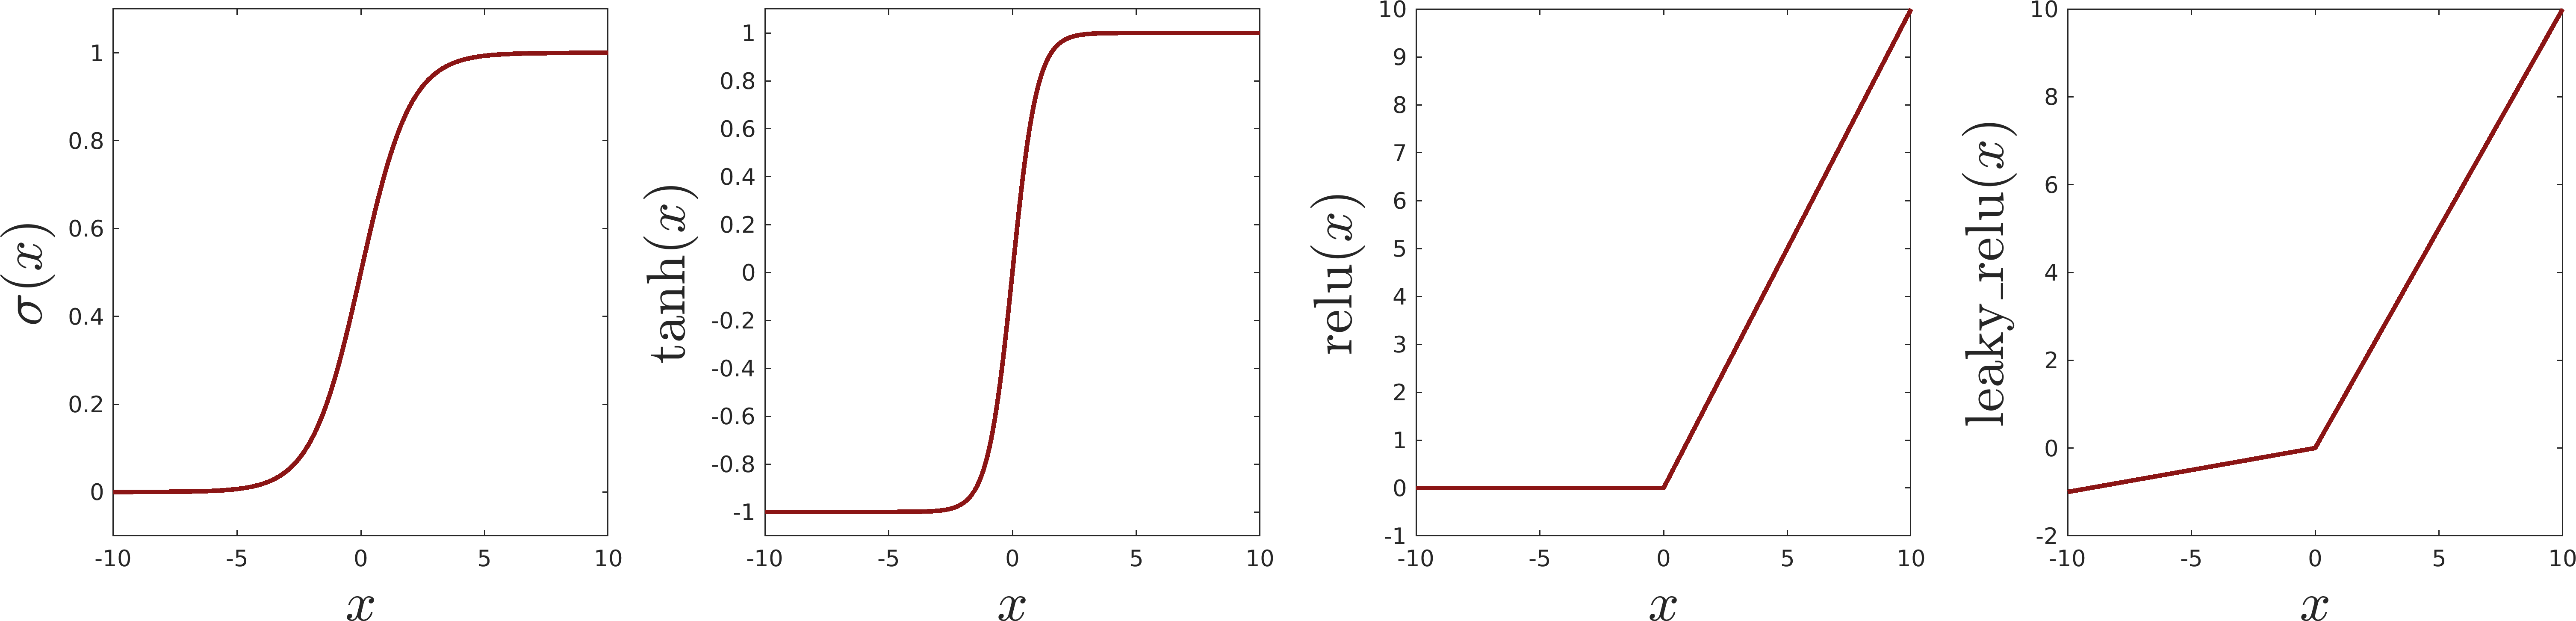
\includegraphics[width=0.95\textwidth]{tex/figs/app01_figs/activations.png}
\caption{Common activation functions used in neural networks.}
\label{fig:activations}
\end{center}
\end{figure*}

It is important to note that each of these activation functions share two important characteristics: they are \textit{nonlinear} and they are easy to differentiate. It is critical that the activation function be nonlinear since a composition of linear functions will remain linear, and therefore no additional benefit is gained in modeling capability by adding more than a single layer to the network. Differentiability is also critical because the gradients must be easily computable during training\footnote{While ReLU and leaky ReLU are not strictly differentiable, this issue is easily mitigated in practice.}.

\subsubsection{Training Neural Networks}
Neural networks are trained with gradient-based numerical optimization techniques, such as those mentioned in Section \ref{subsubsec:MLnumopt} (e.g. stochastic gradient descent). Therefore once a particular loss function $L$ has been chosen, the gradients $\frac{\partial L}{\partial \theta}$ must be computed for each parameter. Since neural networks can contain a large number of parameters, this gradient computation must be accomplished in a computationally efficient way. In particular, the gradients are computed using an algorithm referred to as \textit{backpropagation}, which leverages the chain rule of differentiation and the layered structure of the network.

As with other parametric models, it is very important to avoid overfitting when training neural networks\footnote{It is quite easy to overfit when training neural networks since they have such a large number of parameters.}. This can partially be accomplished using the division of the dataset into training and test sets, as well as by using regularization techniques as mentioned in Section \ref{subsubsec:MLreg}. Another technique for avoiding overfitting in neural networks is referred to as \textit{dropout}, where some ``connections'' in the network are occasionally removed during the training process. This essentially forces the network to learn more redundant representations, which has been shown to improve generalization. Of course another useful technique to avoid overfitting is just to have an extremely large dataset, but in many cases this may not be very practical.

\subsection{Backpropagation and Computational Graphs}
From a theoretical standpoint, computing the gradients $\frac{d L}{d \theta}$ of the loss function with respect to the parameters is relatively straightforward. However, from a practical standpoint computing these gradients can be computationally expensive, especially for complex models such as neural networks.
\textit{Backpropagation}\footnote{Sometimes also referred to as auto-differentiation.} is an algorithm that addresses this issue by computing all required gradients in an efficient way\marginnote{Many software tools, such as PyTorch (\texttt{https://pytorch.org/}) and TensorFlow (\texttt{https://www.tensorflow.org/}) will automatically be able to perform backpropagation for a large class of functions.}. 

Backpropagation computes gradients by cleverly choosing the order in which operations required to compute the gradient are performed. By doing so it seeks to avoid redundant computations, and can in fact be viewed as an example of dynamic programming. While in some simple cases the backpropagation algorithm may provide only a small advantage, in many cases (and in particular for neural network training) backprop can be orders of magnitude faster than naive approaches.

A \textit{computational graph} is another practical tool that is useful when using the backpropagation algorithm to compute gradients. A computational graph provides a way to express a mathematical function using representations from graph theory. In particular the function is expressed as a directed graph where the nodes represent mathematical operations or function inputs and the edges represent intermediate quantities. Using a computational graph, a forward pass through the graph (starting at the root nodes, which are function inputs) is equivalent to evaluating the function.

This representation makes it very easy to see the structure of the mathematical operation that can be exploited by the backpropagation algorithm.
As an example, consider the function $L(x,y) = g(f(x,y))$ and its associated computational graph shown in Figure \ref{fig:backprop} (which includes the intermediate variable $z$). Using the chain rule, the gradient of $L$ with respect to $x$ is $\frac{\partial L}{\partial x} = \frac{dL}{dz}\frac{\partial z}{\partial x}$. The backpropagation algorithm uses this structure to convert the computation of the gradient $\frac{\partial L}{\partial x}$ into a sequence of \textit{local} gradient computations $\frac{dL}{dz}$ and $\frac{\partial z}{\partial x}$, corresponding to each computation node in the graph. With this structure redundant computation can be be avoided. For example, when computing $\frac{\partial L}{\partial y}$ the partial gradient $\frac{dL}{dz}$ can be reused.

\begin{figure}[ht]
\begin{center}
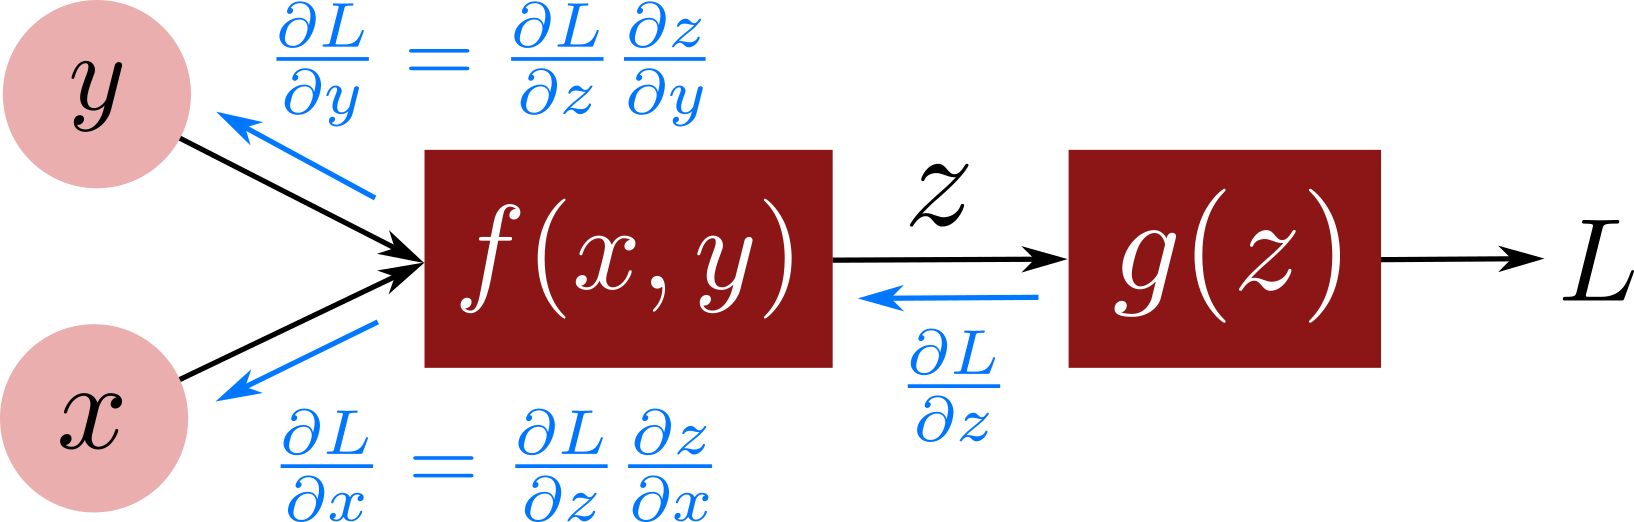
\includegraphics[width=0.55\textwidth]{tex/figs/app01_figs/backprop.png}
\caption{Example computational graph for a function $L(x,y) = g(f(x,y))$.}
\label{fig:backprop}
\end{center}
\end{figure}

To summarize, the backpropagation algorithm follows the following basic steps:
\begin{enumerate}
    \item Perform a forward pass through the computational graph to compute any intermediate variables that may be needed for computing local gradients\footnote{For example if $g(z) = z^2$ the gradient $\frac{dg}{dz} = 2z$ depends on the current value of $z$}.
    \item Starting from the graph output, perform a backwards pass over the graph where at each computation node the local gradient of the node with respect to its inputs and outputs is computed. Then, compute the gradient of the graph's output with respect to the inputs of the local computation node, leveraging the chain rule and previously calculated gradients. In Figure \ref{fig:backprop}, the first step of backprop would be to compute $\frac{\partial L}{\partial z} = \frac{d g}{d z}$, and the second step would use $\frac{\partial L}{\partial z}$ to compute the remaining gradients $\frac{\partial L}{\partial x}$ and $\frac{\partial L}{\partial y}$.
\end{enumerate}




\begin{example}[Training a Simple Model] \label{ex:backprop}
Consider a supervised learning problem with a parametric model defined as:
\begin{equation*}
f(x) = (x+a)(x+b),
\end{equation*}
where $a$ and $b$ are parameters of the model, and a $l_2$ loss function \eqref{eq:l2loss} is used for training. A computational graph for computing the loss from a single data point with this model is shown in Figure \ref{fig:graph}.
\begin{marginfigure}
\begin{center}
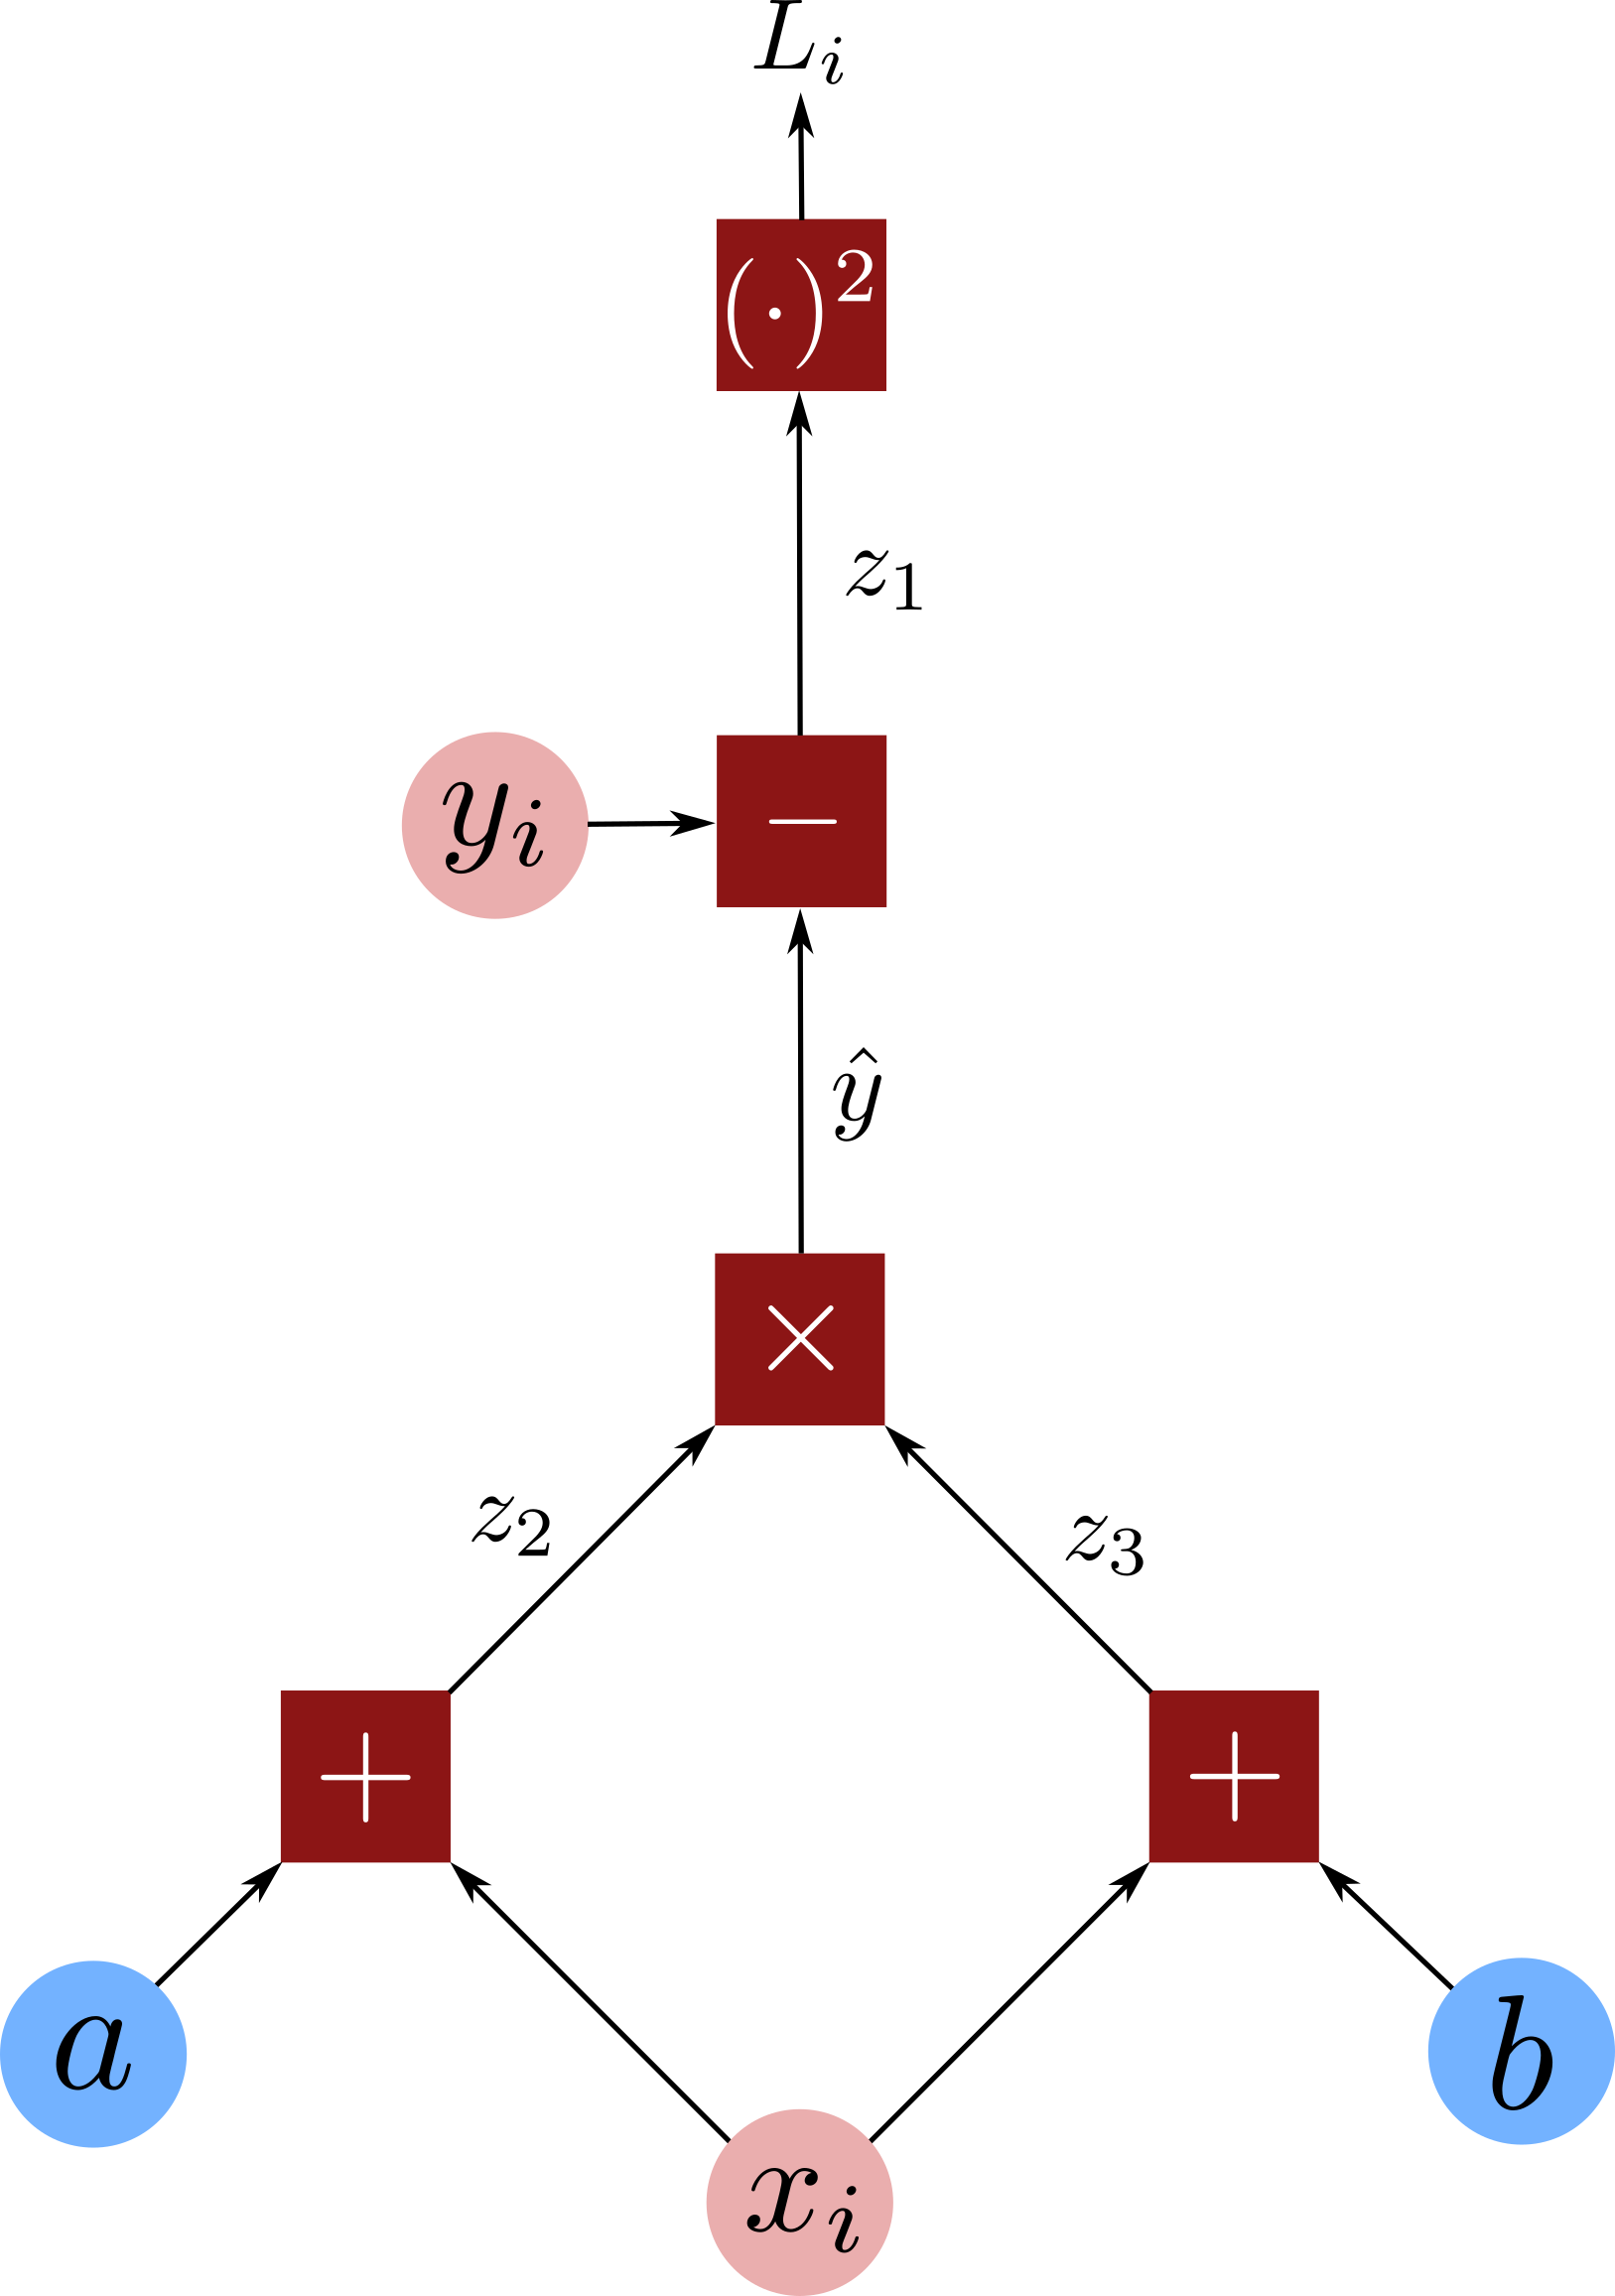
\includegraphics[width=0.95\textwidth]{tex/figs/app01_figs/graph.png}
\caption{Computational graph for computing the loss for a single data point for the model $f(x) = (x+a)(x+b)$ with $l_2$ loss (see Example \ref{ex:backprop}). The values $(x_i, y_i)$ are the data point, the model output is $\hat{y}$, and $z_1$, $z_2$, $z_3$ are intermediate variables. The quantities $a$ and $b$ are parameters of the model.}
\label{fig:graph}
\end{center}
\end{marginfigure}

For this model and loss function the gradients required for training can be computed analytically as:
\begin{equation*}
\begin{split}
\frac{\partial L_i}{\partial a} &= -2(y - (x+a)(x+b))(x+b), \\
\frac{\partial L_i}{\partial b} &= -2(y - (x+a)(x+b))(x+a).\\
\end{split}
\end{equation*}
Computing the gradients in this way (the naive approach) would require $7$ operations each (4 sums and 3 multiplications), for a total of $14$ operations.

Alternatively the gradients can be computed in a more efficient way using backpropagation, which avoids redundant computations. This approach can be viewed as taking a \textit{backward pass} over the computation graph. Starting at the output of the graph:
\begin{equation*}
\begin{split}
\frac{\partial L_i}{\partial z_1} = 2z_1.
\end{split}
\end{equation*}
Then moving on through the next operations and using the chain rule (and reusing the previous computations):
\begin{equation*}
\begin{split}
\frac{\partial L_i}{\partial \hat{y}} = \frac{\partial L_i}{\partial z_1}\frac{\partial z_1}{\partial \hat{y}} = -\frac{\partial L_i}{\partial z_1},
\end{split}
\end{equation*}
and:
\begin{equation*}
\begin{split}
\frac{\partial L_i}{\partial z_2} &= \frac{\partial L_i}{\partial \hat{y}}\frac{\partial \hat{y}}{\partial z_2} = \frac{\partial L_i}{\partial \hat{y}}z_3, \\
\frac{\partial L_i}{\partial z_3} &= \frac{\partial L_i}{\partial \hat{y}}\frac{\partial \hat{y}}{\partial z_3} = \frac{\partial L_i}{\partial \hat{y}}z_2. \\
\end{split}
\end{equation*}
Finally, the next step backward reaches the parameters $a$ and $b$:
\begin{equation*}
\begin{split}
\frac{\partial L_i}{\partial a} &= \frac{\partial L_i}{\partial z_2}\frac{\partial z_2}{\partial a} = \frac{\partial L_i}{\partial z_2}, \\
\frac{\partial L_i}{\partial b} &= \frac{\partial L_i}{\partial z_3}\frac{\partial z_3}{\partial b} = \frac{\partial L_i}{\partial z_3}. \\
\end{split}
\end{equation*}
To actually compute the numerical values of these gradients:
\begin{enumerate}
    \item First perform a forward pass through the network to compute the values $z_1$, $z_2$, and $z_3$ (5 operations).
    \item Then perform the backward pass computations to compute $\frac{\partial L_i}{\partial z_1}$, $\frac{\partial L_i}{\partial \hat{y}}$, $\frac{\partial L_i}{\partial z_2}$, $\frac{\partial L_i}{\partial z_3}$, $\frac{\partial L_i}{\partial a}$, and $\frac{\partial L_i}{\partial b}$ (4 operations).
\end{enumerate}
Using backpropagation, only 9 operations are required to compute the gradients $\frac{\partial L_i}{\partial a}$, and $\frac{\partial L_i}{\partial b}$, which is a non-negligible reduction over the naive approach!



\end{example}